\subsection{CARGA}
\subsubsection{Gráfico de Dependencia}
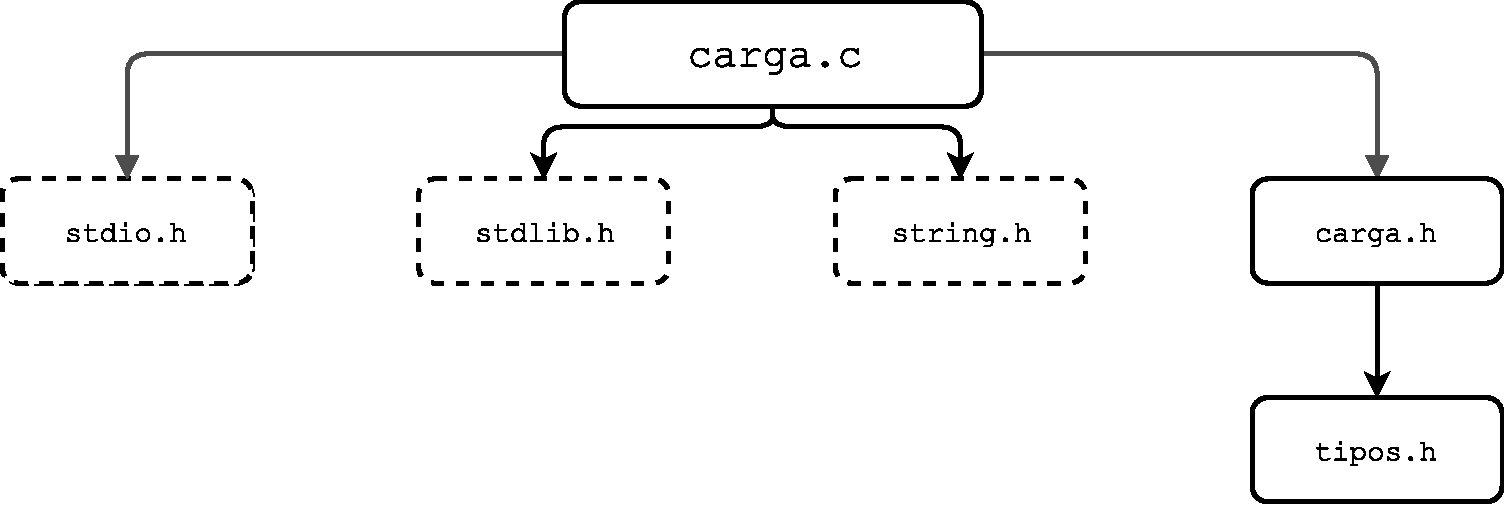
\includegraphics[width=\textwidth, angle=0]{image.pdf}
\subsubsection{Funciones}
\begin{Table}
	\label{mdl:carga}
	\begin{tabular}{rl}
		\sintc & \funref{estadoUsuario(char** c)}{def:estusuario}\\
		\sintc & \funref{perfilUsuario(char** c)}{def:perfilusuario}\\
		\tipos{static}{struct:usuarios}{Usuarios}{*}& \funref{initUsuarios(int* n)}{def:initusuarios}  \\
		\tipos{static}{struct:vehiculos}{Vehiculos}{*}&\funref{initVehiculos(int* n)}{def:initvehiculos}  \\
 		\tipos{static}{struct:viajes}{Viajes}{*}&\funref{initViajes(int* n)}{def:initviajes} \\
 		\tipos{static}{struct:pasos}{Pasos}{*}&\funref{initPasos(int* n)}{def:initpasos} \\
 		\tipos{static}{struct:incidencias}{Incidencias}{*}&\funref{initIncidencias(int* n)}{def:initincidencias} \\
 		\sintc &\funref{idaVuela(char** c)}{def:idavuelta} \\
 		\sintc &\funref{estadoViaje(char** c)}{def:estviaje} \\
 		\sintc &\funref{estadoIncidencia(char** c)}{def:estincidencia} \\
		\cc{void}&\funrf{cargar}{def:cargar}\cc{(Usuarios** usuarios,}\\
				  &\cc{Vehiculos** vehiculos,}\\
				  &\cc{Viajes** viajes,}\\
				  &\cc{Pasos** pasos,}\\
				  &\cc{Incidencias** incidencias,}\\
				  &\cc{int* tam);}
	\end{tabular}
\end{Table}
\subsubsection{Definiciones}
\begin{itemize}
	\item \label{def:cargar}
	\begin{lstlisting}
		void cargar(Usuarios** pUsuarios,
					Vehiculos** pVehiculos,
					Viajes** pViajes,
					Pasos** pPasos,
					Incidencias** pIncidencias,
					int* pInt);
	\end{lstlisting}
	\begin{itemize}
		\item \textbf{Parametros}
		\begin{itemize}
			\item \cc{pUsuarios} $\rightarrow$ Puntero a puntero de usuarios.
			\item \cc{pVehiculos} $\rightarrow$ Puntero a puntero de vehiculos.
			\item \cc{pViajes}$\rightarrow$ Puntero a puntero de viajes.
			\item \cc{pPasos}$\rightarrow$ Puntero a puntero de pasos.
			\item \cc{pIncidencias}$\rightarrow$ Puntero a puntero de incidencias.
			\item \cc{pInt}$\rightarrow$ Puntero a vector para almacenar el tamaño de las estructuras.
		\end{itemize}
	\newpage
	\end{itemize}
	\item \label{def:estincidencia}\cc{int estadoIncidencia(char** c);}
	\begin{itemize}
		\item \textbf{Parametros}
		\begin{itemize}
			\item \cc{c} $\rightarrow$ Recibe una cadena de caracteres por referencia.
			
		\end{itemize}
		\item \textbf{Devuelve}
		\begin{itemize}
			\item $0$ si \cc{c} = \cc{'cerrada'}
			\item $1$ si \cc{c} = \cc{'abierta'}
			\item $2$ si \cc{c} = \cc{'validada'}
		\end{itemize}
	\end{itemize}
	\item\label{def:estusuario}\cc{int estadoUsuario(char** c);}
	\begin{itemize}
		\item \textbf{Parametros}
		\begin{itemize}
			\item \cc{c} $\rightarrow$ Recibe una cadena de caracteres por referencia.
			
		\end{itemize}
		\item \textbf{Devuelve}
		\begin{itemize}
			\item $0$ si \cc{c} = \cc{'bloqueado'}
			\item $1$ si \cc{c} = \cc{'activo'}
		\end{itemize}
	\end{itemize}
	\item\label{def:estviaje}\cc{int estadoViaje(char** c);}
	\begin{itemize}
		\item \textbf{Parametros}
		\begin{itemize}
			\item \cc{c} $\rightarrow$ Recibe una cadena de caracteres por referencia.
			
		\end{itemize}
		\item \textbf{Devuelve}
		\begin{itemize}
			\item $0$ si \cc{c} = \cc{'cerrado'}
			\item $1$ si \cc{c} = \cc{'abierto'}
			\item $2$ si \cc{c} = \cc{'iniciado'}
			\item $3$ si \cc{c} = \cc{'finalizado'}
			\item $4$ si \cc{c} = \cc{'anulado'}
		\end{itemize}
	\end{itemize}
	\item\label{def:idavuelta}\cc{int idaVuelta(char** c);}
	\begin{itemize}
		\item \textbf{Parametros}
		\begin{itemize}
			\item \cc{c} $\rightarrow$ Recibe una cadena de caracteres por referencia.
		\end{itemize}
		\item \textbf{Devuelve}
		\begin{itemize}
			\item $0$ si \cc{c} = \cc{'vuelta'}
			\item $1$ si \cc{c} = \cc{'ida'}
		\end{itemize}
	\end{itemize}
	\item\label{def:initincidencias}\tipos{}{struct:incidencias}{Incidencias}{* initIncidencias(int* n);}
	\begin{itemize}
		\item \textbf{Parametros}
		\begin{itemize}
			\item \cc{n} $\rightarrow$ Referencia a la posición del vector que almacena el número de incidencias.
		\end{itemize}
		\item \textbf{Devuelve}
		\begin{itemize}
			\item Un vector con los datos contenidos en el fichero \textbf{Incidencias.txt}.
		\end{itemize}
	\end{itemize}
	\item\label{def:initpasos}\tipos{}{struct:pasos}{Pasos}{* initPasos(int* n);}
	\begin{itemize}
		\item \textbf{Parametros}
		\begin{itemize}
			\item \cc{n} $\rightarrow$ Referencia a la posición del vector que almacena el número de pasos.
		\end{itemize}
		\item \textbf{Devuelve}
		\begin{itemize}
			\item Un vector con los datos contenidos en el fichero \textbf{Pasos.txt}.
		\end{itemize}
	\end{itemize}
	\newpage
	\item\label{def:initusuarios}\tipos{}{struct:usuarios}{Usuarios}{* initUsuarios(int* n);}
	\begin{itemize}
		\item \textbf{Parametros}
		\begin{itemize}
			\item \cc{n} $\rightarrow$ Referencia a la posición del vector que almacena el número de usuarios.
		\end{itemize}
		\item \textbf{Devuelve}
		\begin{itemize}
			\item Un vector con los datos contenidos en el fichero \textbf{Usuarios.txt}.
		\end{itemize}
	\end{itemize}
	\item\label{def:initvehiculos}\tipos{}{struct:vehiculos}{Vehiculos}{* initVehiculos(int* n);}
	\begin{itemize}
		\item \textbf{Parametros}
		\begin{itemize}
			\item \cc{n} $\rightarrow$ Referencia a la posición del vector que almacena el número de vehiculos.
		\end{itemize}
		\item \textbf{Devuelve}
		\begin{itemize}
			\item Un vector con los datos contenidos en el fichero \textbf{Vehiculos.txt}.
		\end{itemize}
	\end{itemize}
	\item\label{def:initviajes}\tipos{}{struct:viajes}{Viajes}{* initViajes(int* n);}
	\begin{itemize}
		\item \textbf{Parametros}
		\begin{itemize}
			\item \cc{n} $\rightarrow$ Referencia a la posición del vector que almacena el número de viajes.
		\end{itemize}
		\item \textbf{Devuelve}
		\begin{itemize}
			\item Un vector con los datos contenidos en el fichero \textbf{Viajes.txt}.
		\end{itemize}
	\end{itemize}
	\item\label{def:perfilusuario}\cc{int perfilUsuario(char** c);}
	\begin{itemize}
		\item \textbf{Parametros}
		\begin{itemize}
			\item \cc{c} $\rightarrow$ Recibe una cadena de caracteres por referencia.
			
		\end{itemize}
		\item \textbf{Devuelve}
		\begin{itemize}
			\item $0$ si \cc{c} = \cc{'administrador'}
			\item $1$ si \cc{c} = \cc{'usuario'}
		\end{itemize}
	\end{itemize}
\end{itemize}
\newpage




